\mathversion{sans}

\DeclarePairedDelimiter{\ivl}{[\mspace{-4.5mu}(}{)\mspace{-4.5mu}]}

\section{Set Representation}


\section{Preimages Under Real Functions}

\newcommand{\cl}[1]{\overline{\vphantom{i}{#1}}}
\newcommand{\sub}[1]{_{_{#1}}}

XXX: lifts are generally uncomputable, but many specific lifts are computable or approximately computable

XXX: something about computing functions backward by computing inverses forward

XXX: obvious how to do this with invertible functions (though infinite endpoints are a little tricky); not obvious how to do the same with two-argument functions

\subsection{Invertible Primitives}

We consider only strictly monotone functions on $\Re$.
Further on, we recover more generality by using language conditionals to implement \emph{piecewise} monotone functions.

One reason we consider only strictly monotone functions is that they are easy to invert.
Recall that a function is invertible (bijective) if and only if it is injective (one-to-one) and surjective (onto).

\begin{lemma}
\label{lem:monotone-implies-invertible}
If $f : A \to B$ is strictly montone, $f$ is injective.
If $f$ is additionally surjective, $f$ and its inverse are continuous.
\end{lemma}

Preimages under invertible functions can be computed using their inverses.
We are primarily interested in computing preimages under restricted functions.

\begin{lemma}
\label{lem:invertible-function-preimages}
Let $A' \subseteq A$, $B' \subseteq B$, and $f : A \to B$ have inverse $f^{-1} : B \to A$.
Let $f' := restrict~f~A'$. Then
\begin{equation}
	preimage~f'~B'\ =\ A' \i image~f^{-1}~B'
\end{equation}
\end{lemma}

\begin{figure}[!tb]
\centering
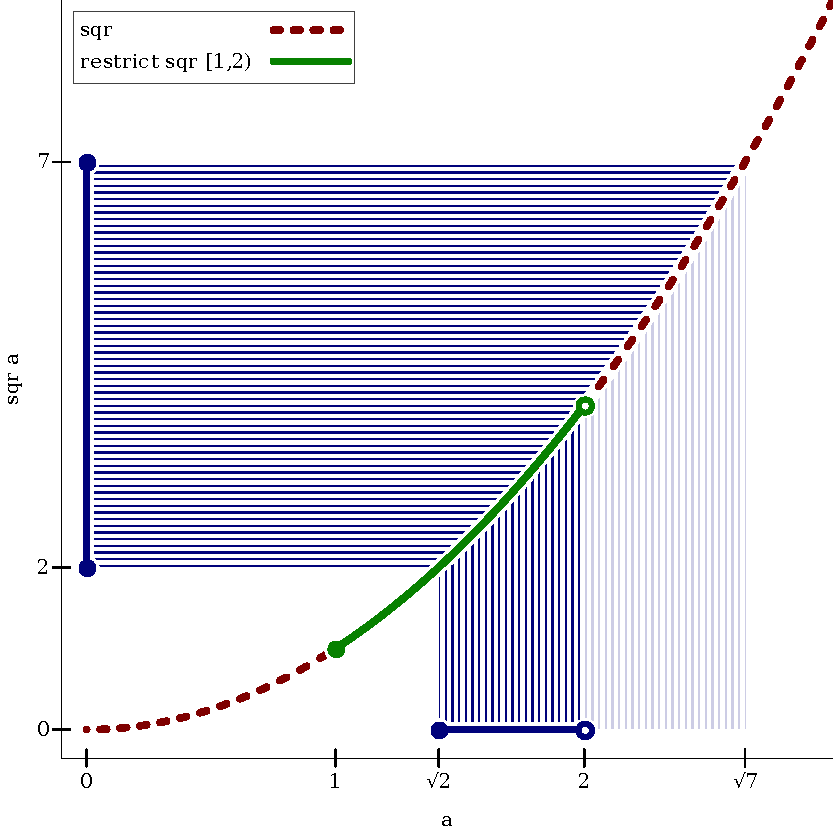
\includegraphics[width=4in]{preimage-by-inverse-image}
\caption[ ]{Computing the preimage of the interval $[2,7]$ under $sqr$ restricted to $[1,2)$, by computing roots and intersecting with $[1,2)$.}
\label{fig:sqr-preimage}
\end{figure}

These facts suggest that we can compute images (or preimages) of intervals under any strictly monotone, surjective $f$ by applying $f$ (or its inverse) to interval endpoints to yield an interval, as in Figure~\ref{fig:sqr-preimage}
This is evident for endpoints in $A$.
Limit endpoints like $+\infty$ require a larger $\cl{f}$ defined on a compact superset of $A$.

The next theorem is easier to state with interval notation in which the kind of interval is not baked into the syntax.

\begin{definition}[interval]
$\ivl{a_1,a_2,\alpha_1,\alpha_2}$ denotes an interval, where $a_1,a_2 \in \cl{\Re}$ are extended real endpoints, and $\alpha_1,\alpha_2 \in Bool$ determine whether $a_1$ and $a_2$ are contained in the interval.
\end{definition}

\begin{example}
Some intervals, using $\ivl{\cdot,\cdot,\cdot,\cdot}$ notation:
\begin{equation}
\begin{aligned}
	\ivl{0,1,true,false} &= [0,1) \\
	\ivl{-\infty,0,false,true} &= (-\infty,0] \\
	\ivl{-\infty,+\infty,false,false} &= (-\infty,+\infty) = \Re \\
	\ivl{-\infty,+\infty,true,true} &= [-\infty,+\infty] = \cl{\Re}
\end{aligned}
\end{equation}
All but the last are subsets of $\Re$.
\exampleqed
\end{example}

\begin{theorem}[images of intervals by endpoints]
\label{thm:images-of-intervals}
Let $\cl{A}$ and $\cl{B}$ be compact subsets of $\cl{\Re}$, $\cl{f} : \cl{A} \to \cl{B}$ strictly monotone and surjective, and $f$ the restriction of $\cl{f}$ to some $A \subseteq \cl{A}$.
For all nonempty $\ivl{a_1,a_2,\alpha_1,\alpha_2} \subseteq A$,
\begin{itemize}
	\item If $\cl{f}$ is increasing, $image~f~\ivl{a_1,a_2,\alpha_1,\alpha_2} = \ivl{\cl{f}~a_1, \cl{f}~a_2,\alpha_1,\alpha_2}$.
	\item If $\cl{f}$ is decreasing, $image~f~\ivl{a_1,a_2,\alpha_1,\alpha_2} = \ivl{\cl{f}~a_2, \cl{f}~a_1,\alpha_2,\alpha_1}$.
\end{itemize}
\end{theorem}
\begin{proof}
Because $\cl{A}$ is compact and totally ordered, every subset of $\cl{A}$ has a lower and an upper bound in $\cl{A}$.
Therefore, the endpoints of every interval subset of $A$ are in $\cl{A}$.

Let $(a_1,a_2] \subseteq A$.
Suppose $\cl{f}$ is strictly increasing; thus $a_1 < a \leq a_2$ if and only if $\cl{f}~a_1 < \cl{f}~a \leq \cl{f}~a_2$, so $image~f~(a_1,a_2] = image~\cl{f}~(a_1,a_2] = (\cl{f}~a_1,\cl{f}~a_2]$.
The remaining cases are similar.
\end{proof}

To use Theorem~\ref{thm:images-of-intervals} to compute preimages under $f$ by computing images under its inverse $f^{-1}$, we must know whether $f^{-1}$ is increasing or decreasing.
The following lemma can help.

\begin{lemma}
\label{lem:inverse-direction}
If $f : A \to B$ is strictly monotone and surjective with inverse $f^{-1} : B \to A$, then $f$ is increasing if and only if $f^{-1}$ is increasing.
\end{lemma}

\begin{example}
The extension of $log : (0,+\infty) \to \Re$ to the compact superdomain $[0,+\infty]$ is defined by
\begin{equation}
\begin{aligned}
	&\cl{log} : [0,+\infty] \to \cl{\Re} \\
	&	\cl{log}~a\ := \lim_{a' \to a} log~a'
		\ =\ \lzfccase{a}{
				0 & -\infty \\
				+\infty & +\infty \\
				else & log~a \\
			}
\end{aligned}
\end{equation}
The extension of its inverse $exp$ is $\cl{exp} : \cl{\Re} \to [0,+\infty]$, defined similarly, which by Lemma~\ref{lem:inverse-direction} is also strictly increasing.
Thus,
\begin{equation}
\begin{aligned}
	image~log~(0,1]\ &=\ (\cl{log}~0,\cl{log}~1] = (-\infty,0]
\\[0.5\baselineskip]
	preimage~log~[0,+\infty)
		\ &=\ image~exp~[0,+\infty)
\\
		\ &=\ [\mspace{2mu}\cl{exp}~0,\cl{exp}~{+\infty})
		= [1,+\infty)
\end{aligned}
\end{equation}
by Theorem~\ref{thm:images-of-intervals} and Lemma~\ref{lem:invertible-function-preimages},
\exampleqed
\end{example}

%%%%%%%%%%%%%%%%%%%%%%%%%%%%%%%%%%%%%%%%%%%%%%%%%%%%%%%%%%%%%%%%%%%%%%%%%%%%%
%%%%%%%%%%%%%%%%%%%%%%%%%%%%%%%%%%%%%%%%%%%%%%%%%%%%%%%%%%%%%%%%%%%%%%%%%%%%%
%%%%%%%%%%%%%%%%%%%%%%%%%%%%%%%%%%%%%%%%%%%%%%%%%%%%%%%%%%%%%%%%%%%%%%%%%%%%%

\subsection{Two-Argument Primitives}

We do not expect to be able to compute preimages under $\Re \times \Re \pto \Re$ primitives by simply inverting them.
Two-argument invertible real functions are difficult to define and are usually pathological.

Instead, we compute approximate preimages only, using inverses with respect to one argument (with the other held constant).

\begin{definition}[axial inverse]
\label{def:axial-inverse}
Let $f_c : A \times B \to C$.
Functions $f_a : B \times C \to A$ and $f_b : C \times A \to B$ defined so that
\begin{equation}
	f_c~\pair{a,b} = c\ \iff\ f_a~\pair{b,c} = a\ \iff\ f_b~\pair{c,a} = b
\end{equation}
are \mykeyword{axial inverses} with respect to $f_c$'s first and second arguments.
\end{definition}

We call $f_c$ \mykeyword{axis-invertible} or \mykeyword{trijective} when it has axial inverses $f_a$ and $f_b$.
We call $f_a$ the \mykeyword{first axial inverse} of $f_c$ because it is the inverse of $f_c$ along the first axis: $f_a$ with only $c$ varying (i.e. $\fun{c \in C} f_a~\pair{b,c}$), is the inverse of $f_c$ with only $a$ varying (i.e. $\fun{a \in A} f_c~\pair{a,b}$).
Similarly, $f_b$ is the \mykeyword{second axial inverse}.

\begin{example}
\label{ex:plus-axial-inverses}
Let $add_c : \Re \times \Re \to \Re$, $add_c~\pair{a,b} := a+b$.
Its axial inverses are $add_a~\pair{b,c} := c - b$ and $add_b~\pair{c,a} := c - a$.
\exampleqed
\end{example}

We have chosen the axial inverse function types carefully: they are the only types for which $f_c$, $f_a$ and $f_b$ form a cyclic group.

\begin{lemma}
\label{lem:axial-inverse-cyclic-group}
The following statements are equivalent.
\begin{itemize}
	\item $f_c$ has axial inverses $f_a$ and $f_b$.
	\item $f_a$ has axial inverses $f_b$ and $f_c$.
	\item $f_b$ has axial inverses $f_c$ and $f_a$.
\end{itemize}
Equivalently, every axis-invertible function generates a cyclic group of order 3 by inversion in the first axis.
\end{lemma}

This fact is analogous to how mutual inverses $f$ and $f^{-1}$ also form a cyclic group (of order 2, generated by inversion).
Similar to using mutual inversion to compute preimages under both $log$ and $exp$, Lemma~\ref{lem:axial-inverse-cyclic-group} allows computing preimages under two-argument functions related by axial inversion.

\begin{example}
Define $sub_c : \Re \times \Re \to \Re$ by $sub_c~\pair{a,b} := a-b$.
Because $sub_c = add_b$, $sub_a = add_c$ and $sub_b = add_a$.
\exampleqed
\end{example}

Unlike inverses, axial inverses do not provide a direct way to compute exact preimages.
Instead, they provide a way to compute a preimage's smallest rectangular bounding set.

\begin{theorem}[preimage bounds from axial inverse images]
\label{thm:axis-invertible-function-preimages}
Let $A' \subseteq A$, $B' \subseteq B$, $C' \subseteq C$, and $f_c : A \times B \to C$ with axial inverses $f_a$ and $f_b$.
If $f_c' = restrict~f_c~(A' \times B')$, then
\begin{equation}
	preimage~f_c'~C'\ \subseteq\ \lzfcsplit{
		&(A' \i image~f_a~(B' \times C'))\ \times \\
		&(B' \i image~f_b~(C' \times A'))}
\end{equation}
Further, the right-hand side is the smallest rectangular superset.
\end{theorem}
\begin{proof}
The smallest rectangle containing $preimage~f_c'~C'$ is
\begin{equation}
	preimage~f_c'~C'\ \subseteq\ 
		\lzfcsplit{
			&(image~fst~(preimage~f_c'~C'))\ \times \\
			&(image~snd~(preimage~f_c'~C'))}
\end{equation}
Starting with the first set in the product, expand definitions, distribute $fst$, replace $f_c~\pair{a,b} = c$ by $f_a~\pair{b,c} = a$, and simplify:
\begin{displaybreaks}
\begin{align*}
	&image~fst~(preimage~f_c'~C')
\nobreak\\
	&\tab =\ image~fst~\setb{\pair{a,b} \in A' \times B'}{f_c~\pair{a,b} \in C'}
\\
	&\tab =\ \setb{a \in A'}{\Exists{b \in B'} f_c~\pair{a,b} \in C'}
\\
	&\tab =\ \setb{a \in A'}{\Exists{b \in B',c \in C'} f_c~\pair{a,b} = c}
\\
	&\tab =\ \setb{a \in A'}{\Exists{b \in B',c \in C'} f_a~\pair{b,c} = a}
\\
	&\tab =\ \setb{f_a~\pair{b,c}}{b \in B', c \in C', f_a~\pair{b,c} \in A'}
\\
	&\tab =\ A' \i \setb{f_a~\pair{b,c}}{b \in B', c \in C'}
\nobreak\\
	&\tab =\ A' \i image~f_a~(B' \times C')
\end{align*}
\end{displaybreaks}
The second set in the product is similar.
\end{proof}

\begin{figure}[!tb]
\centering
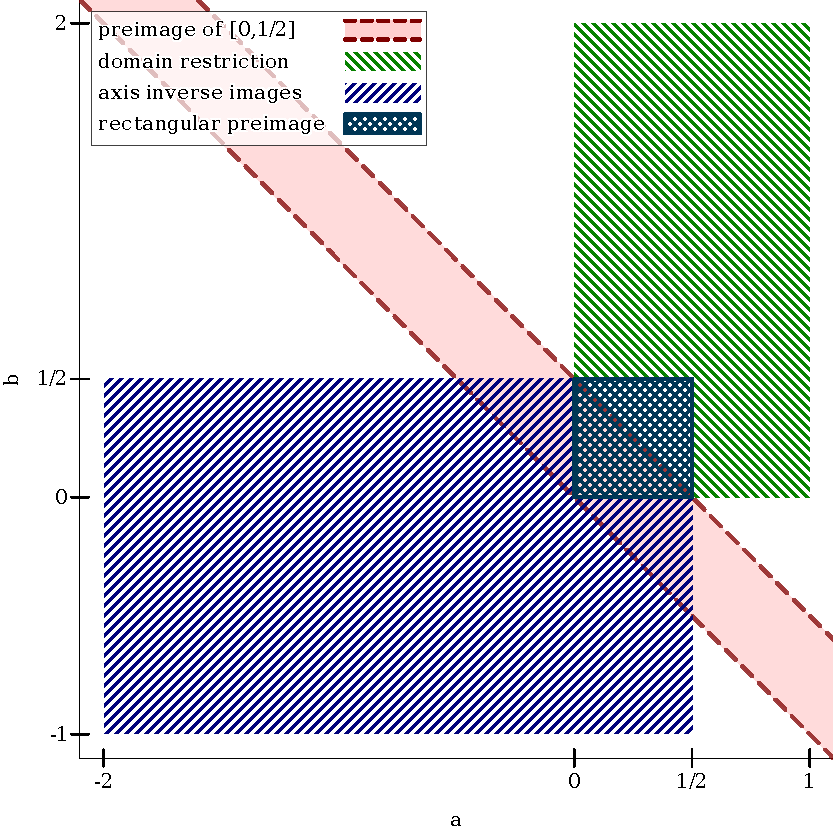
\includegraphics[width=4in]{rect-preimage-by-inverse-images}
\caption[ ]{Computing an approximate preimage of $[0,\tfrac{1}{2}]$ under addition restricted to $[0,1] \times [0,2]$ (Example~\ref{ex:plus-preimage}).
The preimage is approximated by intersecting the domain with an overapproximation computed using axial inverses.}
\label{fig:plus-preimage}
\end{figure}

\begin{example}
\label{ex:plus-preimage}
See Figure~\ref{fig:plus-preimage}.
Let $add_c' := restrict~add_c~([0,1] \times [0,2])$.
By Theorem~\ref{thm:axis-invertible-function-preimages},
\begin{align*}
	preimage~add_c'~[0,\tfrac{1}{2}]
		&\subseteq \lzfcsplit{
			&([0,1] \i image~add_a~([0,2] \times [0,\tfrac{1}{2}]))\ \times \\
			&([0,2] \i image~add_b~([0,\tfrac{1}{2}] \times [0,1]))}
\\
		&= ([0,1] \i [-2,\tfrac{1}{2}]) \times ([0,2] \i [-1,\tfrac{1}{2}])
\\
		&= [0,\tfrac{1}{2}] \times [0,\tfrac{1}{2}]
\end{align*}
is the smallest rectangular subset of $[0,1] \times [0,2]$ that contains the preimage of $[0,\tfrac{1}{2}]$ under $add_c$.
\exampleqed
\end{example}

At this point, we have an analogue of Lemma~\ref{lem:invertible-function-preimages}, in that we can compute (approximate) preimages by computing images under (axial) inverses.
To compute images using interval endpoints, we need analogues of Lemma~\ref{lem:monotone-implies-invertible} (strictly monotone, surjective functions are invertible and continuous), Theorem~\ref{thm:images-of-intervals} (images of intervals by endpoints), and Lemma~\ref{lem:inverse-direction} (inverse direction).

We first need a notion of properties that hold along an axis for every fixed value of the other argument.

\begin{definition}[uniform axis property]
$f_c : A \times B \to C$ has property $P$ \keyword{uniformly} in its first axis when $P~(flip~(curry~f_c)~b)$ for all $b \in B$, and uniformly in its second axis when $P~(curry~f_c~a)$ for all $a \in A$.
If the axis is not specified, $P$ holds uniformly for both.
\end{definition}

Now Lemma~\ref{lem:monotone-implies-invertible}'s analogue is an easy corollary.

\begin{lemma}
\label{lem:uniformly-monotone-implies-invertible}
Let $f_c : A \times B \to C$ for totally ordered $A$, $B$ and $C$.
If $f_c$ is uniformly surjective and either uniformly strictly increasing or uniformly strictly decreasing in each axis, then $f_c$ is axis-invertible; further, it and its axial inverses are continuous.
\end{lemma}

From here on, assume axis monotonicity properties are uniform unless otherwise stated.

\begin{example}
$add_c$ is uniformly surjective and strictly increasing.
$sub_c$ is uniformly surjective and strictly increasing/decreasing in its first/second axis.
Therefore, both are axis-invertible.
\exampleqed
\end{example}

Restriction usually makes a function not uniformly surjective.

\begin{example}
Let $add_c' : [0,1] \times [0,1] \to [0,2]$, defined by restricting $add_c$.
It is strictly increasing, but not uniformly surjective: the range of $curry~add_c'~0$ is $[0,1]$, not $[0,2]$.
\exampleqed
\end{example}

\begin{figure}[!tb]
\centering
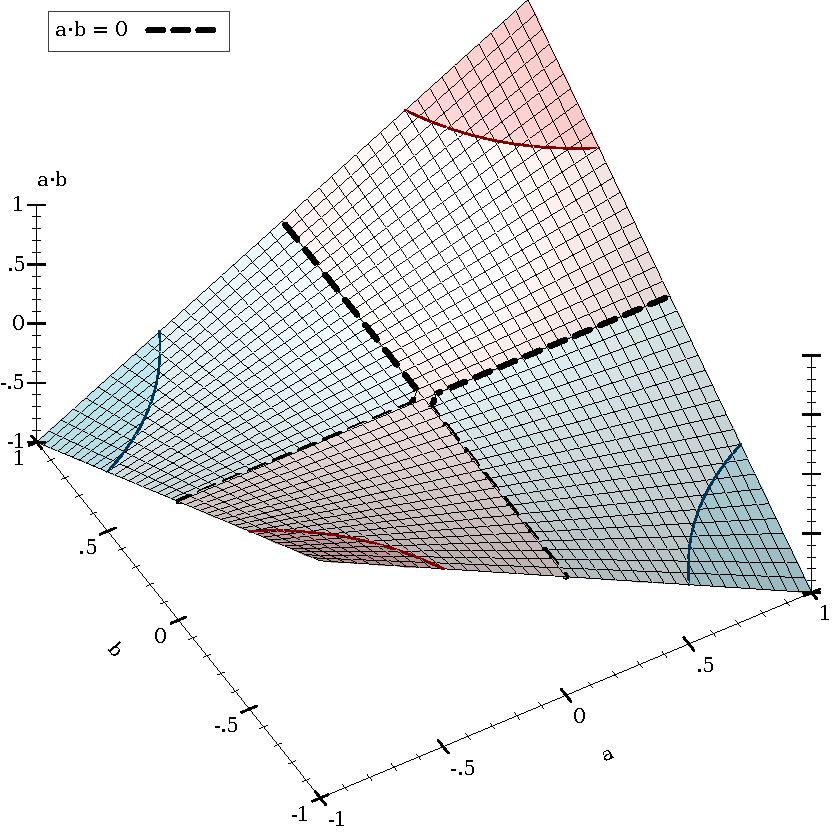
\includegraphics[width=4in]{mul-nonuniform-properties}
\caption[ ]{Multiplication on $\Re \times \Re$ is not uniformly surjective, nor uniformly strictly increasing or decreasing in each axis: $a \cdot 0 = 0$ and $0 \cdot b = 0$ for all $a$ and $b$ (Example~\ref{ex:mul-nonuniform}).
Fortunately, it is uniformly surjective and strictly monotone in each open quadrant.}
\label{fig:mul-nonuniform}
\end{figure}

Fortunately, restriction sometimes does the opposite.

\begin{example}
\label{ex:mul-nonuniform}
Define $mul_c : \Re \times \Re \to \Re$ by $mul_c~\pair{a,b} := a \cdot b$.
It is not uniformly surjective nor strictly monotone because $mul_c~\pair{0,b} = 0$ for all $b \in B$.
(See Figure~\ref{fig:mul-nonuniform}.)
But $mul_c^{++} : (0,+\infty) \times (0,+\infty) \to (0,+\infty)$, and $mul_c$ restricted to the other open quadrants, are uniformly surjective and strictly increasing or decreasing in each axis.
\exampleqed
\end{example}

Theorem~\ref{thm:images-of-intervals} justifies computing images of intervals with infinite endpoints by applying an extended function to the endpoints.
Its two-argument analogue is more involved because extended, two-argument functions may not be defined at every point.

\begin{example}
$add_c$ cannot be extended to $\cl{add_c} : \cl{\Re} \times \cl{\Re} \to \cl{\Re}$ in the same way $log$ is extended to $\cl{log}$ because
\begin{equation}
	\lim_{\pair{a',b'} \to \pair{a,b}} add_c~\pair{a',b'}
\end{equation}
does not exist when $\pair{a,b}$ is $\pair{-\infty,+\infty}$ or $\pair{+\infty,-\infty}$.
\exampleqed
\end{example}

The previous example suggests that extensions of increasing, two-argument functions are always well-defined except at off-diagonal corners.
This is true, and similar statements hold for axes with other directions, and for more restricted domains.

\begin{theorem}[$\cl{\Re} \times \cl{\Re}$ extension]
\label{thm:two-argument-extensions}
Let $A$, $B$, $C$ be open subsets of $\Re$, with $f_c : A \times B \to C$ uniformly surjective and strictly increasing or decreasing in each axis.
Let $\cl{A}$, $\cl{B}$ and $\cl{C}$ be the closures of $A$, $B$ and $C$ in $\cl{\Re}$.
The following extension is well-defined:
\begin{equation}
\begin{aligned}
	&\cl{f_c} : (\cl{A} \times \cl{B}) \w N \to \cl{C} \\
	&\cl{f_c}~\pair{a,b}\ :=\ \lim_{\pair{a',b'} \to \pair{a,b}} f_c~\pair{a',b'}
\end{aligned}
\end{equation}
where $N := \set{\pair{min~\cl{A},max~\cl{B}},\pair{max~\cl{A},min~\cl{B}}}$ if $f_c$ is increasing or decreasing, and
$N := \set{\pair{min~\cl{A},min~\cl{B}},\pair{max~\cl{A},max~\cl{B}}}$ if $f_c$ is increasing/decreasing or decreasing/increasing.
\end{theorem}
\begin{proof}
Suppose $f_c$ is increasing, and let $g : \Nat \to A \times B$ be a sequence of $f_c$'s domain values.

Any $g$ that converges to $\pair{max~\cl{A},max~\cl{B}}$ has a strictly increasing subsequence.
By monotonicity, $map~f_c~g$ has a strictly increasing subsequence.
It is bounded by $max~\cl{C}$, so $\cl{f_c}~\pair{max~\cl{A},max~\cl{B}} = max~\cl{C}$.
A similar argument proves $\cl{f}~\pair{min~\cl{A},min~\cl{B}} = min~\cl{C}$.

For any $g$ that converges to $\pair{max~\cl{A},b'}$ for some $b' \in B$, define
\begin{equation}
	g'\ :=\ map~(\fun{\pair{a,b}}\pair{f_a~\pair{b',f_c~\pair{a,b}}',b'})~g
\end{equation}
where $f_a$ is $f_c$'s first axial inverse, so that $map~f_c~g = map~f_c~g'$.
Because $g'$ has a subsequence that is strictly increasing in the first of each pair, and because the second of each pair is the constant $b'$, by monotonicity, $map~f_c~g'$ has a strictly increasing subsequence.
It is bounded by $max~\cl{C}$, so $\cl{f_c}~\pair{max~\cl{A},b'} = max~\cl{C}$.
By similar arguments, $\cl{f}~\pair{min~\cl{A},b} = min~\cl{C}$ and so on.

Arguments for $f$ decreasing, etc., are similar.
\end{proof}

Following the proof of Theorem~\ref{thm:two-argument-extensions}, extensions of two-argument functions can be defined by two corner cases, four border cases, and an interior case.

\begin{example}
Define $pow_c : (0,1) \times (0,+\infty) \to (0,1)$ by $pow_c~\pair{a,b} := exp~(b \cdot log~a)$, which is increasing/decreasing.
Its extension to a subset of $\cl{\Re} \times \cl{\Re}$ is
\begin{equation}
\begin{aligned}
	&\cl{pow_c} : ([0,1] \times [0,+\infty]) \w N \to [0,1] \\
	&\cl{pow_c}~\pair{a,b}\ :=\
		\lzfccase{\pair{a,b}}{
			\pair{0,+\infty} & 0 \\
			\pair{1,0} & 1 \\ 
			\pair{0,b} & 0 \\
			\pair{1,b} & 1 \\
			\pair{a,0} & 1 \\
			\pair{a,+\infty} & 0 \\
			else & pow_c~\pair{a,b}
		}
\end{aligned}
\end{equation}
where $N := \set{\pair{0,0},\pair{1,+\infty}}$.
\exampleqed
\end{example}

The analogue of Theorem~\ref{thm:images-of-intervals} is easiest to state if we have predicates that indicate a function's direction in each axis.
Define $inc_1 : (A \times B \to C) \tto Bool$ so that $inc_1~f$ if and only if $f$ is strictly increasing in its first axis, and similarly $inc_2$ so that $inc_2~f$ if and only if $f$ is strictly increasing in its second axis.

\begin{theorem}[images of rectangles by interval endpoints]
\label{thm:images-of-rectangles}
Let $A,B,C$ be open subsets of $\Re$, with $f_c : A \times B \to C$ uniformly surjective and strictly increasing or decreasing in each axis, with extension $\cl{f_c}$ as defined in Theorem~\ref{thm:two-argument-extensions}.
If $A' := \ivl{a_1,a_2,\alpha_1,\alpha_2} \subseteq A$ and $B' := \ivl{b_1,b_2,\beta_1,\beta_2} \subseteq B$, then the image $C'$ under $f_c$ is
\begin{equation}
\begin{aligned}
	&image~f_c~(\ivl{a_1,a_2,\alpha_1,\alpha_2} \times \ivl{b_1,b_2,\beta_1,\beta_2})
\\
	&\tab =\ \lzfclet{
		\pair{a_1,a_2,\alpha_1,\alpha_2} & \lzfccond{(inc_1~f_c) & \pair{a_1,a_2,\alpha_1,\alpha_2} \\ else & \pair{a_2,a_1,\alpha_2,\alpha_1}} \\
		\pair{b_1,b_2,\beta_1,\beta_2} & \lzfccond{(inc_2~f_c) & \pair{b_1,b_2,\beta_1,\beta_2} \\ else & \pair{b_2,b_1,\beta_2,\beta_1}}
	}{\ivl{\cl{f_c}~\pair{a_1,b_1},\cl{f_c}~\pair{a_2,b_2},\alpha_1~and~\beta_1,\alpha_2~and~\beta_2}}
\end{aligned}
\end{equation}
\end{theorem}
\begin{proof}
Because $f_c$ is continuous and $A' \times B'$ is a connected set, $C'$ is a connected set, which in $\Re$ is an interval.
Thus, we need to determine only its bounds and whether it contains each endpoint.

Suppose $f_c$ is increasing.
By monotonicity, $C'$ is contained in $[\cl{f_c}~\pair{a_1,b_1},\cl{f_c}~\pair{a_2,b_2}]$.
If either $\alpha_1$ or $\beta_1$ is $false$, $C'$ cannot contain $\cl{f_c}~\pair{a_1,b_1}$.
If either $\alpha_2$ or $\beta_2$ is $false$, $C'$ cannot contain $\cl{f_c}~\pair{a_2,b_2}$.
Therefore $C' = \ivl{\cl{f_c}~\pair{a_1,b_1},\cl{f_c}~\pair{a_2,b_2},\alpha_1~and~\beta_1,\alpha_2~and~\beta_2}$.

We still must prove $\pair{a_1,b_1}$ and $\pair{a_2,b_2}$ are in $\cl{f_c}$'s domain.
First, recall $\cl{f_c} : (\cl{A} \times \cl{B}) \w N \to \cl{C}$, where $\cl{A}$, $\cl{B}$ and $\cl{C}$ are the closures of $A$, $B$ and $C$ in $\cl{\Re}$, and $N = \set{\pair{min~\cl{A},max~\cl{B}},\pair{max~\cl{A},min~\cl{B}}}$.

Because $A' \subseteq A$ and $B' \subseteq B$, and $A$ and $B$ are open sets, $a_1 \neq max~\cl{A}$, $a_2 \neq \min~\cl{A}$, $b_1 \neq max~\cl{B}$, and $b_2 \neq min~\cl{B}$, so
\begin{equation}
\begin{aligned}
	\pair{a_1,b_1} &\neq \pair{max~\cl{A},b} & \text{for all}\ b \in \cl{B} \\
	\pair{a_1,b_1} &\neq \pair{a,max~\cl{B}} & \text{for all}\ a \in \cl{A} \\
	\pair{a_2,b_2} &\neq \pair{min~\cl{A},b} & \text{for all}\ b \in \cl{B} \\
	\pair{a_2,b_2} &\neq \pair{a,min~\cl{B}} & \text{for all}\ a \in \cl{A} \\
\end{aligned}
\end{equation}
Therefore, $\pair{a_1,b_1} \not\in N$ and $\pair{a_2,b_2} \not\in N$, as desired.

The remaining cases for $f_c$ are similar.
\end{proof}

\begin{example}
Because $inc_1~pow_c$ and $not~(inc_2~pow_c)$,
\begin{align*}
	&image~pow_c~((0,\tfrac{1}{2}] \times [2,+\infty))
\\
	&\ =\ \lzfclet{
		\pair{a_1,a_2,\alpha_1,\alpha_2} & \pair{0,\tfrac{1}{2},false,true} \\
		\pair{b_1,b_2,\beta_1,\beta_2} & \pair{+\infty,2,false,true}
	}{\ivl{\cl{pow_c}~\pair{a_1,b_1},\cl{pow_c}~\pair{a_2,b_2},\alpha_1~and~\beta_1,\alpha_2~and~\beta_2}}
\\
	&\ =\ \ivl{\cl{pow_c}~\pair{0,+\infty},\cl{pow_c}~\pair{\tfrac{1}{2},2},false~and~false,true~and~true}
\\
	&\ =\ \ivl{0,\tfrac{1}{4},false,true}
\\
	&\ =\ (0,\tfrac{1}{4}]
\\[-2.25\baselineskip]
\end{align*}
\exampleqed
\end{example}

To use Theorem~\ref{thm:images-of-rectangles} to compute approximate preimages under $f_c$ by computing images under its axial inverses, we must know whether each axis of $f_a$ and $f_b$ is increasing or decreasing.
It helps to have an analogue of Lemma~\ref{lem:inverse-direction} (inverse direction).

\begin{theorem}
Let $f_c : A \times B \to C$ be uniformly surjective and strictly increasing or decreasing in each axis, with axial inverses $f_a$ and $f_b$.
The following statements hold:
\begin{enumerate}
	\item $inc_1~f_a$ if and only if $(inc_1~f_c)~xor~(inc_2~f_c)$.
	\item $inc_2~f_a$ if and only if $inc_1~f_c$.
\end{enumerate}
\end{theorem}
\begin{proof}
For statement 1, let $c \in C$, $b_1,b_2 \in B$, $a_1 := f_a~\pair{b_1,c}$ and $a_2 := f_a~\pair{b_2,c}$.
Let $c' := f_c~\pair{a_1,b_2}$; note $c = f_c~\pair{a_1,b_1} = f_c~\pair{a_2,b_2}$.
Suppose $inc_1~f_c$ and $inc_2~f_c$; then $a_1 > a_2 \iff c < c'$ and $b_1 < b_2 \iff c < c'$, so $b_1 < b_2 \iff a_1 > a_2$.
The remaining cases are similar.

For statement 2, fix $b \in B$ and apply Lemma~\ref{lem:inverse-direction}.
\end{proof}

By Lemma~\ref{lem:axial-inverse-cyclic-group}, $inc_1~f_b \iff inc_2~f_c$, and $inc_2~f_b \iff inc_1~f_a$.
We can therefore easily determine the uniform directions of $f_a$'s and $f_b$'s axes from the uniform directions of $f_c$'s axes.

We are certain the preceeding definitions and theorems extend naturally to functions with any number of arguments, but have not needed to extend them yet.

%%%%%%%%%%%%%%%%%%%%%%%%%%%%%%%%%%%%%%%%%%%%%%%%%%%%%%%%%%%%%%%%%%%%%%%%%%%%%
%%%%%%%%%%%%%%%%%%%%%%%%%%%%%%%%%%%%%%%%%%%%%%%%%%%%%%%%%%%%%%%%%%%%%%%%%%%%%
%%%%%%%%%%%%%%%%%%%%%%%%%%%%%%%%%%%%%%%%%%%%%%%%%%%%%%%%%%%%%%%%%%%%%%%%%%%%%

\subsection{Discontinuous Primitives}

\section{Primitive Implementation}
\label{sec:primitive-implementation}

Because floating-point functions are defined on subsets of $\cl{\Re}$, it would seem we could compute preimages under strictly monotone, real functions by applying their floating-point counterparts to interval endpoints.
This is mostly true, but we must take care to round in the right directions and account for floating-point negative zero.

\begin{equation}
\begin{aligned}
	&\cl{pos!recip} : [0,+\infty] \to [0,+\infty] \\
	&\cl{pos!recip}~a\ =\
		\lzfccond{
			0 < a < +\infty & 1/a \\
			a = 0 & +\infty \\
			a = +\infty & 0
		}
\end{aligned}
\end{equation}

\section{Partitioned Sampling}

Suppose that we want to sample values in a probability space $X,P$ by first sampling a set from a \emph{partition} of $X$ and then sampling from that set.\footnote{This is not \emph{stratified} sampling, which samples a fixed number of times from each partition.}
[XXX: this transition should mention why we want to do partition sampling instead of just supposing that we do]

First, we define
\begin{equation}
\begin{aligned}
	&condition : Set~X \pto [0,1] \tto Set~X \tto Set~X \pto [0,1] \\
	&condition~P~A\ :=\ \fun{A' \in domain~P} P~(A' \i A)~{/}~P~A
\end{aligned}
\end{equation}
to restrict a probability measure $P$ to a measurable, positive-probability set $A$ and renormalize it.

\begin{definition}[partitioned sampling]
\label{def:partitioned-sampling}
Let $X,P$ be an arbitrary probability space, $N$ be an at-most-countable index set, and $s : N \to Set~X$ be a partition of $X$ into $|N|$ measurable parts. The following procedure samples from $X$:
\begin{enumerate}
	\item Choose $n \in N$ with probability $P~(s~n)$.
	\item Choose $a \in s~n$ according to $condition~P~(s~n)$.
\end{enumerate}
\end{definition}

It is not hard to show that partitioned sampling chooses an $a \in X$ according to $P$.

\begin{example}[partitioned sampling from a standard normal]
\label{ex:partitioned-sampling}
Let $P$ be the standard normal distribution's probability measure.
To sample according to $P$, let $N := \set{neg,pos}$ and $s = [neg \mapsto (-\infty,0], pos \mapsto (0,+\infty)]$, and define $Q : N \to Set~\Re \pto [0,1]$ by
\begin{equation}
\begin{aligned}
	Q~neg~A\ &=\ P~((-\infty,0] \i A)~{/}~\tfrac{1}{2} \\
	Q~pos~A\ &=\ P~((0,+\infty) \i A)~{/}~\tfrac{1}{2}
\end{aligned}
\end{equation}
Then
\begin{enumerate}
	\item Choose $n = neg$ or $n = pos$, each with probability $\frac{1}{2}$.
	\item Choose $a \in s~n$ according to $Q~n$.\exampleqed
\end{enumerate}
\end{example}

Partitioned sampling has two weaknesses.
First, it requires $P~(s~n)$ to be easy to compute for all $n \in N$.
If this were true, we would not need to sample in the first place---i.e. it assumes a solution to the overall problem we are trying to solve.
Second, it assumes sampling according to $condition~P~(s~n)$ is easy, which is also not reasonable, as sampling according to a conditioned distribution is a subproblem we are trying to solve.

But suppose we could easily sample a partition index according to a different distribution over $N$, and according to a different distribution over part $s~n$ for each $n \in N$. Doing so and returning weighted samples to adjust for the differences in distribution comprises \mykeyword{partitioned importance sampling}.

First, we define
\begin{equation}
\begin{aligned}
	&subcond : Set~X \pto [0,1] \tto Set~X \tto Set~X \pto [0,1] \\
	&subcond~P~A\ :=\ \fun{A' \in domain~P} P~(A' \i A)
\end{aligned}
\end{equation}
to restrict a probability measure $P$ to a measurable set $A$ \emph{without} renormalizing it; i.e. it returns a subprobability measure.

\begin{definition}[partitioned importance sampling]
\label{def:partitioned-importance-sampling}
Suppose we have
\begin{itemize}
	\item An arbitrary probability space $X,P$.
	\item An at-most-countable index set $N$.
	\item A probability mass function $p : N \to [0,1]$ such that $p~n > 0$ for all $n \in N$.
	\item A partition $s : N \to Set~X$ of $X$ into $|N|$ measurable parts.
	\item Candidate probability measures $Q : N \to Set~X \pto [0,1]$, one for each partition.
\end{itemize}
To sample from $X$ according to $P$,
\begin{enumerate}
	\item Choose $n \in N$ with probability $p~n$.
	\item Choose $a \in X$ according to $Q~n$.
	\item Compute $w := \dfrac{1}{p~n} \cdot diff^+~(subcond~P~(s~n))~(Q~n)~a$.
	\item Return the weighted sample $\pair{a,w}$.
\end{enumerate}
\end{definition}

The function $diff^+~(subcond~P~(s~n))~(Q~n)$, with type $X \to [0,+\infty)$, is a \keyword{Radon-Nikod\'ym\footnote{Pronounced ``RADon neekohDIM,'' and named after Austrian mathematician Johann Radon and Polish mathematician Otto Nikod\'ym.} derivative}.
If $P$ has density $f$, $Q~n$ has density $g$ with respect to the same base measure (e.g. same-dimensional length, area or volume), and $a \in s~n$ implies $g~a > 0$, then\footnote{The equality holds $(Q~n)$-almost everywhere.}
\begin{equation}
	diff^+~(subcond~P~(s~n))~(Q~n)~a\ =\ if~(a \in s~n)~(f~a~{/}~g~a)~0
\end{equation}
Chapter~\ref{ch:sampling-algorithm-proofs} has definitions and more details.
We use $diff^+$ in a more general sense, but in this section, it is usually fine to think of its return values as quotients of densities.

An importance sampling algorithm is correct when all expected values computed using its weighted samples are the equal to the true expected values.
The next theorem states that this is true of partitioned importance sampling under reasonable conditions, which are analogous to the support of $subcond~P~(s~n)$ being no larger than that of $Q~n$.

\begin{theorem}[partitioned importance sampling correctness]
\label{thm:partitioned-importance-sampling-correctness}
Let $X$, $P$, $N$, $s$, $p$, and $Q$ as in Definition~\ref{def:partitioned-importance-sampling} (partitioned importance sampling) such that $subcond~P~(s~n) \ll Q~n$ for all $n \in N$. Define $P_N : Set~N \to [0,1]$ by extending $p$ to a measure.

If $g : X \to \Re$ is a $P$-integrable mapping, and
\begin{equation}
\begin{aligned}
	&g' : N \times X \to \Re \\
	&g'~\pair{n,a}\ :=\ g~a \cdot \dfrac{1}{p~n} \cdot diff^+~(subcond~P~(s~n))~(Q~n)~a
\end{aligned}
\end{equation}
then $int~g'~(P_N \times Q)~(N \times X)\ =\ int~g~P~X$.
\end{theorem}
\begin{proof}
See Chapter~\ref{ch:sampling-algorithm-proofs}.
\end{proof}

Partitioned importance sampling allows quite a lot of freedom: parts can be chosen with arbitrary nonzero probability, and each part can have its own candidate distribution, which may be defined on a superset of the part.

\begin{figure}[!tb]
\centering
\subfloat[Unweighted samples]{
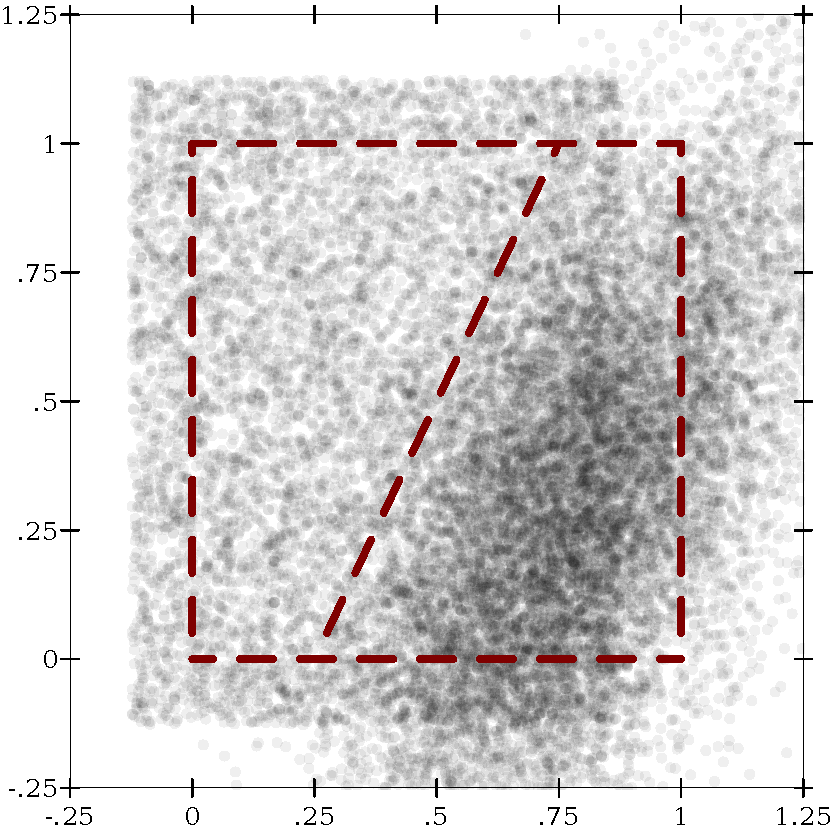
\includegraphics[width=3in]{pimp-sampling-unweighted}
}
\hspace{0.1in}
\subfloat[Resampled by weight]{
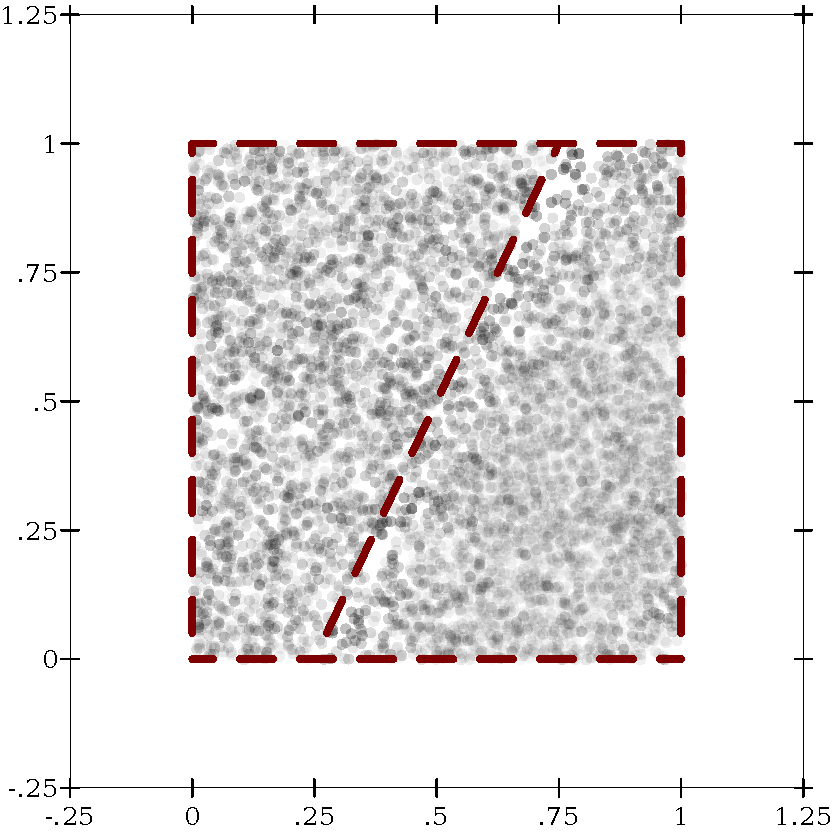
\includegraphics[width=3in]{pimp-sampling-weighted}
}
\caption[ ]{Partitioned importance sampling used to sample uniformly in a partition of the unit square, using two overlapping candidate distributions.}
\label{fig:pimp-sampling-2d}
\end{figure}

\begin{example}[2D partitioned importance sampling]
\figref{fig:pimp-sampling-2d} shows the result of partitioned importance sampling in a partition of the unit square.
In this instance,
\begin{itemize}
	\item $X := [0,1] \times [0,1]$ and $P$ is the uniform measure on $X$ (i.e. area).
	\item $N := \set{left,right}$.
	\item $p := [left \mapsto 0.4, right \mapsto 0.6]$.
	\item $s~left = \setb{\pair{x,y} \in X}{y > 2 \cdot x - \frac{1}{2}}$, similarly for $s~right$.
	\item $Q~left$ is the uniform measure on a superset of $s~left$, and $Q~right$ is a multivariate Gaussian measure centered at $\pair{0.8,0.3}$.
\end{itemize}
The implementation does not actually construct most of these objects. It constructs
\begin{itemize}
	\item A density function $f : \Re \times \Re \tto [0,+\infty)$ to represent $P$.
	\item A family of predicates $s? : N \tto X \tto Bool$ to decide $a \in s~n$.
	\item Candidate densities $g : N \tto X \tto [0,+\infty)$ to represent $Q$.
\end{itemize}
It computes weights using $diff^+~(subcond~P~(s~n))~(Q~n)~a\ =\ f~a~{/}~g~n~a$ when $s?~n~a = true$.
It directly represents only $N$ and $p$, but we will find even this to be infeasible shortly.
\exampleqed
\end{example}

Two properties make the preceeding example simple.
First, the partition has finitely many parts.
Second, the measures $subcond~P~(s~n)$ and $Q~n$ have densities with respect to the same base measure, which ensures $diff^+~(subcond~P~(s~n))~(Q~n)$ exists and is easy to compute.

When sampling in the domain of programs, neither property holds in general.

\subsection{Partitioning Probabilistic Program Domains}

For the random source part $R := J \to [0,1]$ of probabilistic language domains, which consists of infinite binary trees of reals, it is not clear that Theorem~\ref{thm:partitioned-importance-sampling-correctness} is applicable.
The main problem is that infinite-dimensional Radon-Nikod\'ym derivatives do not generally exist.

Fortunately, they \emph{can} exist if the two measures differ in only finitely many axes.
More precisely, let $P_1 : Set~R \to [0,1]$ and $P_2 : Set~R \to [0,1]$ be probability measures, and $J' \subseteq J$ be a finite set of tree indexes.
Suppose $P_1$ can be factored into a distribution $P_1'$ over $J' \to [0,1]$ and a distribution over $(J \w J') \to [0,1]$, and $P_2'$ can be similarly factored into $P_2'$ and \emph{the same} distribution over $(J \w J') \to [0,1]$.
Then, under reasonable conditions (which are analogous to the support of $P_1'$ being no larger than that of  $P_2'$), $diff^+~P_1~P_2$ exists and can be computed using $diff^+~P_1'~P_2'$.
Chapter~\ref{ch:sampling-algorithm-proofs} contains a formal statement of this fact and a proof.

To ensure $subcond~P~(s~n)$ and $Q~n$ differ in only finitely many axes, we partition $R$ according to branch traces.
Each branch trace corresponds with a program that reads any $r \in R$ at only finitely many indexes $J' \subseteq J$.
[XXX: connect idea better]

In the remainder of this subsection, assume a fixed program $\mathit{p}$. Let $f := \meaningofconv{\mathit{p}}_\pbot : \pair{\pair{R,T},\pair{}} \pbotto Y$ be its interpretation as a bottom* arrow computation, with maximal domain $A^*$.
Define $T^* := image~(fst~\arrowcomp~snd)~A^*$ as its \mykeyword{maximal branch trace set} and
$R^* := image~(fst~\arrowcomp~fst)~A^*$ as its \mykeyword{maximal random source set}.

We need a notion of the random sources that agree with a given branch trace $t \in T$; i.e. those $r \in R$ for which $f~\pair{\pair{r,t},\pair{}} \neq \bot$.

\begin{definition}[induced random sources]
\label{def:induced-random-sources}
Let $t \in T$ be a branch trace. The \mykeyword{random sources induced by $t$} are a subset of $R$ defined by
$R' := \setb{r \in R}{\pair{\pair{r,t},\pair{}} \in A^*}$.
%\begin{equation}
	%image~(fst~\arrowcomp~fst)~(preimage~(g~((R \times \set{t}) \times X))~Y)
%\end{equation}
\end{definition}

[XXX: graph of induced partition from program $if~(random < random)~true~false$?]

Using $T$ as the partition index set and defining the partition's parts as induced random sources \emph{almost} works, in the sense that the required Radon-Nikod\'ym derivatives exist.
Unfortunately, we cannot use $T$ or $T^*$ as the partition index set because many branch traces can induce the same random sources.

\begin{example}
For the program
\begin{equation}
	if~(random < p)~0~random
\end{equation}
there are at least two branch traces in the program's maximal domain: $t_0 := [j_0 \mapsto true, * \mapsto \bot]$ and $t_1 := [j_0 \mapsto false, * \mapsto \bot]$.
There is also $[j_0 \mapsto false, left~j_0 \mapsto true, * \mapsto \bot]$, because it agrees with every execution that $[j_0 \mapsto false, * \mapsto \bot]$ agrees with.
In fact, there are infinitely many branch traces in $T^*$ that induce the same random sources as either $t_0$ or $t_1$.
[XXX: tree diagrams?]
\exampleqed
\end{example}

We need to find a subset of branch traces whose induced random sources are disjoint.
The main idea is to define equivalence classes of branch traces that induce the same random sources, and use the ``smallest'' branch trace in each class as a part index.

First, we need to be sure that such equivalence classes can induce a partition.

\begin{theorem}
Let $t_1,t_2 \in T^*$.
If $t_1$ induces $R_1'$ and $t_2$ induces $R_2'$, then $R_1' = R_2'$ or $R_1' \i R_2' = \emptyset$.
\end{theorem}
\begin{proof}
XXX: do this
\end{proof}

To identify the ``smallest'' trace in each class, we must define an ordering over them.
One fairly natural way is to say a branch trace is smaller than another when it describes fewer branch decisions; i.e. its tree has fewer non-$\bot$ elements.
Two branch traces that differ by returning respectively $true$ and $false$ for the same $j$ may represent different execution paths, so they must be incomparable.

\begin{definition}[brach trace partial order]
$t_1 \leq t_2$ when for all $j \in J$, if $t_1~j \neq t_2~j$, then $t_1~j = \bot$.
\end{definition}

If $T^*$ is partitioned into equivalence classes of traces that induce the same random sources, each part in the partition contains a least member with respect to $(\leq)$.

\begin{theorem}
Let $t \in T^*$ induce $R'$, and let $T'$ be the largest subset of $T^*$ that induces $R'$.
$T'$ has a least member $t_*$.
\end{theorem}
\begin{proof}
Define $t_* \in T$ by
\begin{equation}
	t_*\ :=\ \lzfccond{
		\Forall{t' \in T'} t'~j = true & true \\
		\Forall{t' \in T'} t'~j = false & false \\
		else & \bot}
\end{equation}
Thus, $t_* \leq t'$ for all $t' \in T'$, or $t_*$ is a lower bound for $T'$.

Let $r \in R'$.
By construction, every conditional subcomputation at index $j \in J$ agrees with $t_*~j$.
Therefore $f~\pair{\pair{r,t_*},\pair{}} \neq \bot$, so $\pair{\pair{r,t_*},\pair{}} \in A^*$, and thus $t_* \in T'$.
\end{proof}

An easy consequence is $T' = \setb{t' \in T^*}{t_* \leq t'}$. [XXX: is it easy?]
Thus, each least member represents a set of larger branch traces that induce the same set of random sources.

We can get our sought-after index set by defining the set of smallest branch traces.

\begin{definition}[minimal branch traces]
The set of \mykeyword{minimal branch traces} $T_*$ is the set of minimal elements in $T^*$, or
\begin{equation}
	T_*\ :=\ \setb{t_1 \in T^*}{\Forall{t_2 \in T^*} t_2 \leq t_1 \implies t_2 = t_1}
\end{equation}
\end{definition}

\begin{theorem}
\label{thm:minimal-induces-partition}
$T_*$ induces a partition of $R^*$.
\end{theorem}
\begin{proof}
XXX: todo
\end{proof}

We can infer from Theorem~\ref{thm:minimal-induces-partition} that a program's minimal branch trace set $T_*$ contains only the actual branches taken when running the program on every $r \in R^*$.
Therefore, one way to sample from $T_*$ with the correct probability---at least, for programs that halt with probability $1$---would be to choose an $r \in R$ uniformly, and run the program on $r$ while recording each branch decision.

But this sampling scheme has problems similar to those of partitioned sampling (Definition~\ref{def:partitioned-sampling}).
First, it assumes the probabilities of branch traces, which are the probabilities of the $R^*$ subsets they induce, are easy to compute.
Second, we are interested in sampling from an \emph{arbitrarily low-probability subset} of $R^*$, which may be covered by the partition induced by an \emph{arbitrarily low-probability subset} of $T_*$.

It appears we have a chicken-and-egg problem, in that
\begin{enumerate}
	\item Sampling in a small subset of $R^*$ requires sampling in a small subset of $T_*$.
	\item Sampling in a small subset of $T_*$ requires sampling in a small subset of $R^*$.
\end{enumerate}
Fortunately, if we allow ourselves subsets of a slightly larger set than $T_*$, and allow ourselves to sample within overapproximating \emph{covers} of $R^*$ subsets, we can use approximate preimage computation to sample from $T_*$ and $R^*$ subsets simultaneously.

\subsection{Approximate Partitions of Probabilistic Program Domains}

We first define the set of branch traces that is slightly larger than $T_*$.

The idea is to define a set of \emph{feasible} branch traces $T_+$ that is derived only from the \emph{shape} of a program, not its actual executions.
We must then ensure that every additional branch trace (i.e. every $t \in T_+ \w T_*$) induces $\emptyset$, so that $T_+$ induces a partition.
After that, we define an algorithm for sampling from $T_+$, which does not require running a probabilistic program on any $r \in R$, and prove the algorithm correct.
We can then extend this algorithm to use preimage computation to sample in arbitrarily good approximations of small subsets of $T_*$ and $R^*$.

\begin{figure*}[!tb]\centering
\smallmathfont
\subfloat[Branch index arrow. Computations return a lazy tree of type $Idxs$, of feasible branch decisions, ignoring the actual values of $if$ conditions. The arrow is directly implementable in any $\lambda$-calculus.]{
\begin{minipage}{0.98\textwidth}
\begin{align*}
\begin{aligned}[t]
	&\begin{aligned}[t]
		Idxs \ ::= &\ \pair{} \gor \pair{Idxs,Idxs} \\
					&\gor if!idxs~J~(1 \tto Idxs)~(1 \tto Idxs) \\
	\end{aligned} \\
\\[-6pt]
	&\begin{aligned}[t]
		&\arrowarr\pbi : (x \tto y) \tto (J \tto Idxs) \\
		&\arrowarr\pbi~f~j\ :=\ \pair{}
	\end{aligned} \\
\\[-6pt]
	&\begin{aligned}[t]
		&(\arrowcomp\pbi) : (J \tto Idxs) \tto (J \tto Idxs) \tto (J \tto Idxs) \\
		&(k_1~\arrowcomp\pbi~k_2)~j \ :=\ \pair{k_1~(left~j), k_2~(right~j)}
	\end{aligned} \\
\\[-6pt]
	&\begin{aligned}[t]
		&(\arrowpair\pbi) : (J \tto Idxs) \tto (J \tto Idxs) \tto (J \tto Idxs) \\
		&(k_1~\arrowcomp\pbi~k_2)~j \ :=\ \pair{k_1~(left~j), k_2~(right~j)}
	\end{aligned} \\
\end{aligned}
&\tab\tab\tab
\begin{aligned}[t]
	&\begin{aligned}[t]
		&\arrowif\pbi : (J \tto Idxs) \tto (J \tto Idxs) \tto (J \tto Idxs) \tto (J \tto Idxs) \\
		&\arrowif\pbi~k_1~k_2~k_3~j \ := \ 
			\lzfclet{
				idxs_2 & \fun{0} k_2~(left~(right~j)) \\
				idxs_3 & \fun{0} k_3~(right~(right~j))
			}{\pair{k_1~j, if!idxs~j~idxs_2~idxs_3}}
	\end{aligned} \\
\\[-6pt]
	&\begin{aligned}[t]
		&\arrowlazy\pbi : (1 \tto (J \tto Idxs)) \tto (J \tto Idxs) \\
		&\arrowlazy\pbi~k~j \ := \ k~0~j
	\end{aligned} \\
\\[-6pt]
	&\begin{aligned}[t]
		&random\pbi : J \tto Idxs \\
		&random\pbi~j \ := \ \pair{}
	\end{aligned} \\
\end{aligned}
\end{align*}
\vspace{3pt}
\hrule
\end{minipage}
\label{fig:collecting-semantics:arrow}
}

\subfloat[The $\lzfclang$ function $traces$ turns a lazy tree of feasible branch decisions into a set of feasible branch traces.]{
\begin{minipage}{0.98\textwidth}
\begin{equation}
\begin{aligned}
	&traces : Idxs \tto Set~T
\\
	&traces~idxs\ :=\ \U_{n \in \Nat} traces^*~n~idxs~[* \mapsto \bot]
\\[6pt]
	&traces^* : \Nat \tto Idxs \tto T \tto Set~T
\\
	&\lzfcsplit[@{}l@{}l@{}]{
	&traces^*~n~\pair{}~t&\ :=\ \set{t}
\\
	&traces^*~n~\pair{idxs_1,idxs_2}~t&\ :=\ 
		\lzfclet{
			T' & traces^*~n~idxs_1~t
		}{\U_{t' \in T'} traces^*~n~idxs_2~t'}
\\
	&traces^*~0~(if!idxs~j~idxs_2~idxs_3)~t&\ :=\ \set{t}
\\
	&traces^*~n~(if!idxs~j~idxs_2~idxs_3)~t&\ :=\ 
		\lzfcsplit{
			&traces^*~(n-1)~(idxs_2~0)~t[j \mapsto true]\ \u \\
			&traces^*~(n-1)~(idxs_3~0)~t[j \mapsto false]\ \u \\
			&\set{t}}
	}
\end{aligned}
\end{equation}
\vspace{3pt}
\hrule
\end{minipage}
\label{fig:collecting-semantics:traces}
}

\subfloat[The stochastic function $sample!trace$ samples $t$ from the set returned by $traces$, and returns $t$ and its probability. It is directly implementable in any $\lambda$-calculus with probabilistic choice.]{
\begin{minipage}{0.98\textwidth}
\begin{equation}
\begin{aligned}
	&sample!trace : Idxs \to \pair{\Re,T}
\\
	&sample!trace~idxs\ :=\ sample!trace^*~idxs~\pair{1,[* \mapsto \bot]}
\\[6pt]
	&sample!trace^* : Idxs \tto \pair{\Re,T} \tto \pair{\Re,T}
\\
	&\lzfcsplit[@{}l@{}l@{}]{
		&sample!trace^*~\pair{}~pt &\ :=\ pt
\\
		&sample!trace^*~\pair{idxs_1,idxs_2}~pt &\ :=\ 
			\lzfclet{
				pt' & sample!trace^*~idxs_1~pt
			}{sample!trace^*~idxs_2~pt'}
\\
		&sample!trace^*~(if!idxs~j~idxs_2~idxs_3)~\pair{p_t,t} &\ :=\ 
			\lzfclet{
				\pair{p_b,b} & sample!branch~\set{true,false,\bot} \\
				pt' & \pair{p_t \cdot p_b, t[j \mapsto b]}
			}{\lzfccase{b}{
				true & sample!trace^*~(idxs_2~0)~pt' \\
				false & sample!trace^*~(idxs_3~0)~pt' \\
				\bot & pt'
				}
			}
	}
\end{aligned}
\end{equation}
\vspace{3pt}
\hrule
\end{minipage}
\label{fig:collecting-semantics:sample-trace}
}

\caption[]{Branch index collecting semantics.}
\label{fig:collecting-semantics}
\end{figure*}

Defining $T_+$ in terms of a program's abstract branching shape requires an additional nonstandard interpretation.
\figref{fig:collecting-semantics:arrow} defines the \mykeyword{branch index} arrow.
Its type is $J \tto Idxs$, which does not refer to a domain or codomain type of program values because its computations do not receive or compute program values.
Instead, they build lazy trees of possible branching decisions, ignoring the actual values of $if$ conditions.
For example, lifted, pure functions are interpreted as $\fun{j} \pair{}$, which takes the function's computation index and returns no decisions.
Composition and pairing of subcomputations $k_1$ and $k_2$ both return $\pair{k_1~(left~j),k_2~(right~j)}$: a node with two children that contain the feasible branch decisions in their subcomputations.

Only $ifte\pbi$ does more than simple structural recursion: it returns $if!idxs~j~idxs_2~idxs_3$ to represent a decision at computation index $j$.
The children $idxs_2$ and $idxs_3$ are lazy, abstract representations of the $if$'s branches.
Like a concrete execution, a branch trace sampler is expected to compute and recur through only one of them.

\figref{fig:collecting-semantics:traces} defines the function $traces$, which transforms these lazy trees of type $Idxs$ into sets of branch traces.
To ensure $trace$ always terminates, it is defined using a depth-limited helper function, which it calls with every depth $n \in \Nat$, and collects the results in a countable union.
It is thus unimplementable, but we will use it only to precisely define the range of a random value.

We define a program's feasible branch traces using the standard first-order semantic function $\meaningofconv{\cdot}_a$ with arrow $a = idxs^*$.

\begin{definition}[feasible branch traces]
A program $\mathit{p}$'s \mykeyword{feasible branch traces} are those in the set $T_+ := traces~(\meaningofconv{\mathit{p}}\pbi~j_0)$.
\end{definition}

If we are to sample $t \in T_+$ and then sample within the $R'$ induced by $t$, we must ensure that $T_+$ includes $T_*$ and induces a partition.

\begin{theorem}
Let $t \in T$ induce $R'$. $R' \neq \emptyset$ if and only if $t \in T^*$. [XXX: needed?]
\end{theorem}
\begin{proof}
$R' \neq \emptyset$ if and only if there is an $r \in R'$ such that $\pair{\pair{r,t},\pair{}} \in A^*$.
\end{proof}

\begin{theorem}
For all $t \in T_+$, either $t \in T_*$ or $t$ induces $\emptyset$.
\end{theorem}
\begin{proof}
XXX: todo
\end{proof}

\begin{corollary}
$T_+$ induces a partition of $R^*$.
\end{corollary}

XXX: now we define a stochastic procedure for sampling in $T_+$

XXX: apologize for being less precise (e.g. stochastic procedures look like $\lzfclang$ but aren't; we assume every operation is lifted to receive a random source as input, etc.)

XXX: suppose we have a stochastic procedure $sample!branch : Set~Bool_\bot \tto \pair{\Re,Bool_\bot}$, where $sample!branch~B$ returns any member of $B$ with some nonzero, constant probability

\figref{fig:collecting-semantics:sample-trace} defines $sample!trace$, a stochastic procedure defined in terms of $sample!branch$.
Given an $idxs : Idxs$, it returns a member of $traces~idxs$ and its probability.
In other words, for a program $\mathit{p}$, the probability that $\pair{p_t,t} = sample!trace~(\meaningofconv{\mathit{p}}\pbi~j_0)$ is $p_t$, and $t \in T_+$.
Further, every $t \in T_+$ has a constant, nonzero probability of being chosen.

Of course, we must prove these facts.

XXX: move the following soundness and completeness proofs to Chapter 10, or define $T_+$ in terms of $sample!trace$ to make the proofs unnecessary; whether the latter will work (or whether it will work better) will probably become clear when I do the missing proof above

\begin{theorem}[$sample!trace^*$ soundness]
For all $t \in T$ and $idxs: Idxs$, there exists an $n \in \Nat$ such that $snd~(sample!trace^*~idxs~\pair{p_t,t}) \in traces^*~n~idxs~t$.
\end{theorem}
\begin{proof}
By structural induction on $Idxs$.

Case $idxs = \pair{}$.
For all $n \in \Nat$, these two statements are equivalent by substituting definitions of $sample!trace^*$ and $traces^*$:
\begin{equation}
\begin{aligned}
	snd~(sample!trace^*~\pair{}~\pair{p_t,t}) &\in traces^*~n~\pair{}~t \\
	t &\in \set{t}
\end{aligned}
\end{equation}

Case $idxs = \pair{idxs_1,idxs_2}$.
Let
\begin{equation}
\begin{aligned}
	\pair{p_t',t'}&\ :=\ sample!trace^*~idxs_1~\pair{p_t,t} \\
	\pair{p_t'',t''}&\ :=\ sample!trace^*~idxs_2~\pair{p_t',t'}
\end{aligned}
\end{equation}
as in the definition of $sample!trace^*$.
By hypothesis, there exists an $n' \in \Nat$ such that $t' \in traces^*~n'~idxs_1~t$.
Again by hypothesis, there exists an $n'' \in \Nat$ such that $t'' \in traces^*~n''~idxs_2~t'$.
Let $n := max~n'~n''$.

Case $idxs = if!idxs~j~idxs_2~idxs_3$.
Let
\begin{equation}
\begin{aligned}
	\pair{p_b,b}&\ :=\ sample!branch~\set{true,false,\bot} \\
	pt' &\ :=\ \pair{p_t \cdot p_b, t[j \mapsto b]}
\end{aligned}
\end{equation}
as in the definition of $sample!trace^*$, and let $\pair{p_t',t'}\ =\ pt'$.
If $b = true$, by hypothesis, there exists an $n' \in \Nat$ such that $snd~(sample!trace^*~(idxs_2~0)~pt') \in traces^*~n'~(idxs_2~0)~t'$; similarly for $b = false$. Let $n := n' + 1$, so $n' = n - 1$.
If $b = \bot$, then $t' = t$, and $t \in \set{t}$ for all $n \in \Nat$.
\end{proof}

\begin{corollary}[$sample!trace$ soundness]
For all $idxs : Idxs$, $snd~(sample!trace~idxs) \in traces~idxs$.
\end{corollary}

\begin{theorem}[$sample!trace^*$ completeness]
For all $idxs : Idxs$, $t \in T$ and $n \in \Nat$, $t' \in traces^*~n~idxs~t$ implies $Pr[snd~(sample!trace^*~idxs~\pair{p_t,t}) = t'] > 0$ (or just $Pr[t'] > 0$).
\end{theorem}
\begin{proof}
By structural induction on $Idxs$.

Case $idxs = \pair{}$.
By definition of $traces^*$, $t' \in traces^*~n~\pair{}~t$ if and only if $t' \in \set{t}$, or $t' = t$.
By definition of $sample!trace^*$, $Pr[snd~(sample!trace^*~idxs~\pair{p_t,t}) = t] = 1$.

Case $idxs = \pair{idxs_1,idxs_2}$.
Let
\begin{equation}
\begin{aligned}
	T'&\ :=\ traces^*~n~idxs_1~t \\
	T''&\ :=\ \U_{t' \in T'} traces^*~n~idxs_2~t'
\end{aligned}
\end{equation}
as in the definition of $traces^*$. Let
\begin{equation}
\begin{aligned}
	\pair{p_t',t'}&\ :=\ sample!trace^*~idxs_1~\pair{p_t,t} \\
	\pair{p_t'',t''}&\ :=\ sample!trace^*~idxs_2~\pair{p_t',t'}
\end{aligned}
\end{equation}
as in the definition of $sample!trace^*$.
Suppose $t'' \in T''$.
Then there exists a $t' \in T'$ such that $t'' \in traces^*~n~idxs_2~t'$.
By hypothesis, $Pr[t'] > 0$, therefore by hypothesis, $Pr[t''] > 0$.

Case $idxs = if!idxs~j~idxs_2~idxs_3$.
Let
\begin{equation}
\begin{aligned}
	\pair{p_b,b}&\ :=\ sample!branch~\set{true,false,\bot} \\
	pt' &\ :=\ \pair{p_t \cdot p_b, t[j \mapsto b]}
\end{aligned}
\end{equation}
as in the definition of $sample!trace^*$, and let $\pair{p_t',t'}\ =\ pt'$.

If $n = 0$, then let
\begin{equation}
\begin{aligned}
	T'&\ :=\ traces^*~0~idxs~t = \set{t}
\end{aligned}
\end{equation}
as in the definition of $traces^*$.
Suppose $t' \in T'$, equiv. $t' = t$, so $Pr[t'] > 0$ iff $Pr[t] > 0$.
Because $Pr[b = \bot] > 0$ and $t[j \mapsto \bot] = t$, $Pr[t] > 0$.

If $n > 0$, then expand $traces^*~n~idxs~t$ to
\begin{equation}
\begin{aligned}
	T_{true}'&\ :=\ traces^*~(n-1)~(idxs_2~0)~t[j \mapsto true]
\\
	T_{false}'&\ :=\ traces^*~(n-1)~(idxs_3~0)~t[j \mapsto false]
\\
	T_\bot'&\ :=\ \set{t}
\\
	T'&\ :=\ T_{true}' \u T_{false}' \u T_\bot'
\end{aligned}
\end{equation}
as in the definition of $traces^*$.
Suppose $t' \in T'$.
If $t' \in T_{true}'$, then because $Pr[b = true] > 0$, by hypothesis, $Pr[t'] > 0$; similarly for $t' \in T_{false}'$ and $t' \in T_\bot'$.
\end{proof}

\begin{corollary}[$sample!trace$ completeness]
For all $idxs : Indx$, $t \in traces~idxs$ implies $Pr[snd~(sample!trace~idxs) = t] > 0$.
\end{corollary}

\begin{theorem}[$sample!trace^*$ correctness]
Let $idxs : Idxs$, $t \in T_+$, $p_t \in [0,1]$, and $\pair{p_t',t'} := sample!trace^*~idxs~\pair{p_t,t}$.
If $Pr[t] = p_t$, then $Pr[t'] = p_t'$.
\end{theorem}
\begin{proof}
By structural induction on $Idxs$.

Case $idxs = \pair{}$.
By definition of $sample!trace^*$, $\pair{p_t',t'} = \pair{p_t,t}$.
Clearly $Pr[t] = p_t$ implies $Pr[t'] = p_t'$.

Case $idxs = \pair{idxs_1,idxs_2}$.
Let
\begin{equation}
\begin{aligned}
	\pair{p_t',t'}&\ :=\ sample!trace^*~idxs_1~\pair{p_t,t} \\
	\pair{p_t'',t''}&\ :=\ sample!trace^*~idxs_2~\pair{p_t',t'}
\end{aligned}
\end{equation}
as in the definition of $sample!trace^*$.
By hypothesis, $Pr[t] = p_t$ implies $Pr[t'] = p_t'$, which (by hypothesis) implies $Pr[t''] = p_t''$.

Case $idxs = if!idxs~j~idxs_2~idxs_3$.
Let
\begin{equation}
\begin{aligned}
	\pair{p_b,b}&\ :=\ sample!branch~\set{true,false,\bot} \\
	pt' &\ :=\ \pair{p_t \cdot p_b, t[j \mapsto b]}
\end{aligned}
\end{equation}
as in the definition of $sample!trace^*$, and let $\pair{p_t',t'}\ =\ pt'$.
By definition of $sample!branch$, $Pr[b] = p_b$.
Because $b$ and $t$ are independently chosen and $t'$ can be generated by no other execution path, $Pr[t'] = Pr[t] \cdot Pr[b] = p_t \cdot p_b$.
If $b = true$, then in $\pair{p_t'',t''} := sample!trace^*~(idxs_2~0)~pr'$, by hypothesis, $Pr[t''] = p_t''$; similarly for $b = false$.
\end{proof}

\begin{corollary}[$sample!trace$ correctness]
If $\pair{p_t,t} := sample!trace~idxs$, then $Pr[t] = p_t$.
\end{corollary}

XXX: sampling from a \emph{subset} of $T_+$ that induces a part of the partition of $R^*$:
\begin{equation}
\begin{aligned}
	&sample!part : Idxs \tto \pair{\Re,Rect~\pair{R,T}} \tto \pair{\Re,Rect~\pair{R,T}} \\
	&\lzfcsplit{
	&sample!part~idxs~\pair{p,R \times T}\ := \\
	&\tab
	\lzfccase{\pair{idxs, \pair{p, refine~(R \times T)}}}{
		\pair{\pair{}, pr} & pr
\\
		\pair{\pair{idxs_1,idxs_2}, pr} &
			\lzfclet{
				pr' & sample!part~idxs_1~pr
			}{sample!part~idxs_2~pr'}
\\
		\pair{if!idxs~j~idxs_2~idxs_3, \pair{p,R \times T}} &
			\lzfclet{
				\pair{p_b,b} & sample!branch~(proj~j~T) \\
				pr' & \pair{p \cdot p_b, R \times unproj~j~T~\set{b}}
			}{\lzfccase{b}{
				true & sample!part~(idxs_2~0)~pr' \\
				false & sample!part~(idxs_3~0)~pr' \\
				\bot & \pair{p \cdot p_b,\emptyset}
				}
			}
	}
	}
\end{aligned}
\end{equation}

XXX: sampling a weighted point from $Rect~\pair{R,T}$:
\begin{equation}
\begin{aligned}
			\lzfclet{
				\pair{r,q} & sample!point~R \\
				t & \The{t \in T} \Forall{t' \in T} t \leq t' \\
				b & f~\pair{\pair{r,t},\pair{}} \\
				w & if~(b \in B)~(1~{/}~p \cdot 1~{/}~q)~0
			}{\pair{r,w}}
\end{aligned}
\end{equation}

XXX: the least $t \in T$, or $\The{t \in T} \Forall{t' \in T} t \leq t'$, is easy to compute: set each unrestricted axis to $\bot$

XXX: decide what theorems are needed and prove them

XXX: extension: interval splitting

XXX: extension: sampling a weighted point using refinement

XXX: extension: not sampling any decision as $\bot$ when sampling in $T_+$; characterize the programs for which this extension doesn't terminate; explain options to detect or fix

\mathversion{normal}
